\documentclass[letterpaper,12pt]{article}

\usepackage[top=1in, left=1.25in, right=1.25in, bottom=1in]{geometry}
\usepackage[utf8]{inputenc}
\usepackage[T1]{fontenc}
\usepackage[spanish]{babel}
\usepackage{graphicx}
\usepackage{caption}
\usepackage{float}
\usepackage[backend=biber,style=numeric,sorting=none]{biblatex}
\usepackage{amsmath}
\addbibresource{bib/referencias.bib}
\usepackage{subcaption}

\begin{document}

\tableofcontents
\clearpage

\section{Introducción}

\begin{itemize}
\item \textbf{Planteamiento del Problema:} Se busca implementar un menú gráfico el cual permita añadir a una lista distintos objetos junto con su precio, así como eliminarlos de distinta manera, buscando simular el carro de compras de una tienda física o de aplicaciones en línea.

\item \textbf{Motivación:} En esta práctica aprenderemos a encapsular objetos para protegerlos de modificaciones involuntarias o acceso a datos para brindarle mayor seguridad al programa, así como a empaquetar los códigos para una mayor organización y control.

\item \textbf{Objetivos:} Implementar un programa que simule el carrito de compras de una tienda digital, mostrando en todo momento la lista completa de objetos dentro del carrito; encapsulando tanto el carrito como los artículos que contiene para controlar de mejor manera su obtención y adición, y empaquetando el código para una mayor organización y seguridad.


\end{itemize}
\section{Marco Teórico}
    \begin{itemize}
        \item \textbf{Encapsulamiento: } El \textit{Encapsulamiento} es el principio de restringir el acceso directo a los atributos de una clase, de modo que solo puedan ser modificados mediante métodos controlados como getters y setters. Este enfoque nos ayuda a proteger los datos, evita inconsistencias y brinda mayor control del programa.~\cite{Encapsulamiento}
        \item \textbf{Modificadores de acceso: } En java se utilizan distintos niveles de visibilidad para reforzar el encapsulamiento. Por ejemplo: el modificador \textit{private} oculta los atributos de cualquier acceso externo a la clase, \textit{public} los expone sin restricciones. Esta jerarquía de accesibilidad otorga flexibilidad al momento de diseñar clases más seguras y modulares.~\cite{Encapsulamiento}
        \item \textbf{Métodos privados y abstracción: } El encapsulamiento también se extiende a métodos, que pueden declararse \textit{private} si solo deben ser utilizados dentro de la propia clase. Esto nos permite ocultar cálculos internos o procedimientos auxiliares, exponiendo unicamente métodos públicos que definen la interfaz.~\cite{Encapsulamiento}
        \item \textbf{Atributos (private final): } Decalarar un atributo como \textit{private final }significa que es un dato privado al que solo es accesible dentro de la clase y es constante después de inicializare, debe recibir un valor en el momento de su declaración o en el constructor de la clase, y no puede modificarse posteriormente.~\cite{Private}
        \item \textbf{Paquetes: } Los paquetes (también conocidos como "package") son una forma de organizar las clases relacionadas en espacios de nombres, de modo que el proyecto gane modularidad, claridad y una mejor estructura.
        Cada archivo fuente Java puede empezar con una línea \textit{package nombredelpaquete; } indicando en qué paquetes se encuentra la clase. Esto permite acceder a esa clase desde fuera del paquete.~\cite{Paquetes}
        
        
    \end{itemize}

\section{Desarrollo}
\textbf{Librerías, clases, paso de mensajes y empaquetado de clases:}
Para esta práctica se implementó un sistema que simula un carrito de comprar con una interfaz gráfica. Para ello, se utilizaron dos librerías:
\begin{enumerate}
    \item \textbf{javax.swing.*} : En este paquete se incluyen las clases necesarias para crear una interfaz gráfica de usuario, permite además crear ventanas, botones, listas y campos de texto.
    \item \textbf{java.awt.event.*} : Proporcionan clases para manejar el diseño de la ventana y los eventos.
\end{enumerate}

Todas las clases han sido organizadas o empaquetadas dentro de la carpeta: \textbf{/mx/unam/fi/poo/p56/}, al agregar: \textbf{package mx.unam.fi.poo.p56;} al inicio de cada clase. 

La clase \textbf{Articulo} representa un objeto genérico del carrito, contiene los atributos \textbf{nombre} y \textbf{precio}. También se implementaron métodos getters para acceder a estos valores y un método \textbf{toString()} que devuelve una cadena con el nombre y el precio del artículo. De este modo, en la interfaz gráfica al agregar un artículo se mostrará en un formato especificado.

En la clase \textbf{Carrito} se utiliza un \textbf{ArrayList} para almacenar los objetos de la clase Articulo, cuenta con varios métodos:
\begin{itemize}
    \item \textbf{agregar(Articulo a)} : Recibe un objeto de tipo Articulo, antes de agregarlo a la lista, verifica que no sea null y que el nombre no este vacío, de ser así devuelve false, en caso de ser válido se agrega a la lista con \textbf{articulos.add(a)} y devuelve true y se agrega a la lista.
    \item \textbf{eliminarPorIndice(int index)} : Recibe un número entero que representa la posición del artículo en la lista. Valida que el índice sea mayor o igual a 0 y que no se pase del tamaño actual de la lista con \textbf{articulos.size()}. Si el índice es válido, elimina el artículo en esa posición con \textbf{articulos.remove(index)} y devuelve true. Si el índice no es válido, devuelve false.
    \item \textbf{eliminarPorNombre(String nombre)} : Recibe una cadena que representa el nombre del artículo a eliminar. Valida que el nombre no sea null ni vacío. Recorre la lista completa con un ciclo \textbf{for} y compara el nombre de cada artículo con el nombre ingresado, ignorando mayúsculas y minúsculas con \textbf{equalsIgnoreCase}. Si encuentra coincidencia, utiliza \textbf{remove(i)} para eliminar ese artículo de la lista y devuelve true, de lo contrario devuelve false.
    \item \textbf{limpiar()} : Elimina todos los artículos de carrito usando \textbf{articulos.clear()}.
    \item \textbf{getArticulos()} : Este devuelve una copia de la lista de artículos, protegiendo así a la lista original de modificaciones externas.
    \item \textbf{getTotal()} : Recorre todos los artículos en la lista sumando sus precios al utilizar un ciclo \textbf{for} para acumular el valor de cada artículo, para ello, hace uso del método \textbf{getPrecio} de la clase Articulo, por último devuelve el precio total.
\end{itemize}
Finalmente la clase \textbf{MainApp} que contiene el metodo main, comienza creando un objeto de la clase Carrito para almacenar los artículos y otro de la clase Vista para representar la ventana de una aplicación. Posteriormente mediante listeners, cada botón de la vista se conecta con la lógica del carrito: 
\begin{itemize}
    \item \textbf{Botón agregar} : Toma los valores escritos en los campos de texto, crea un nuevo Articulo, lo agrega al carrito y lo muestra en la lista de la ventana.
    \item \textbf{Botón Eliminar seleccionado} : Detecta el artículo marcado en la lista y lo elimina tanto de la vista como del carrito.
    \item \textbf{Botón Eliminar por nombre} : Pide al usuario el nombre de un artículo mediante un cuadro de diálogo y elimina los artículos que coincidan.
    \item \textbf{Botón Limpiar carrito} : Vacía completamente el carrito y actualiza la interfaz de la vista.
\end{itemize}


\clearpage

\section{Resultados}

\begin{figure}[H]
    \centering
    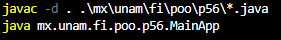
\includegraphics[width=0.7\linewidth]{Imagenes/comp.png}
    \caption*{Compilación y ejecución usando paquetes}
\end{figure}

\begin{figure}[H]
    \centering
    \begin{subfigure}{0.45\textwidth}
        \centering
        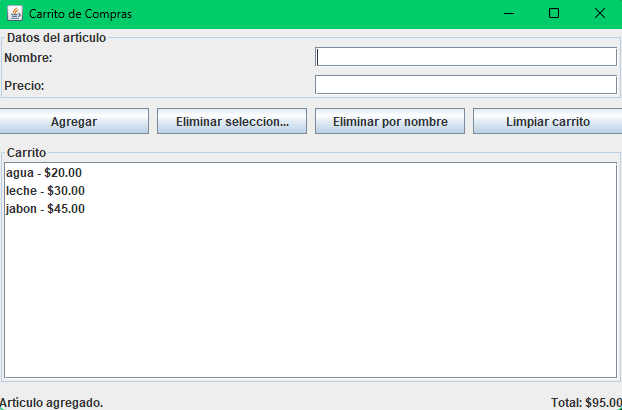
\includegraphics[width=\linewidth]{Imagenes/agregar.png}
        \caption*{Agregar artículos al carrito}
    \end{subfigure}
    \hfill
    \begin{subfigure}{0.45\textwidth}
        \centering
        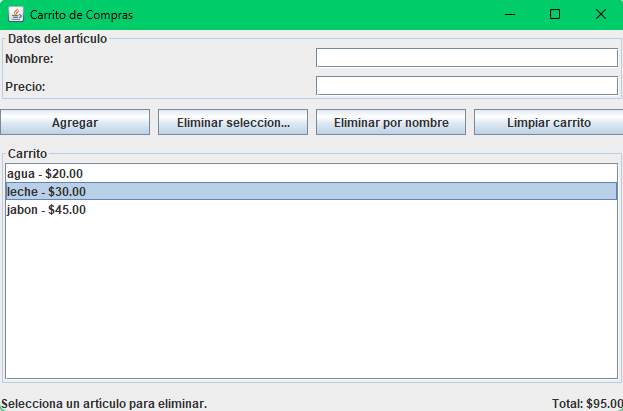
\includegraphics[width=\linewidth]{Imagenes/seleccion.png}
        \caption*{Eliminar artículos por selección}
    \end{subfigure}
\end{figure}

\begin{figure}[H]
    \centering
    \begin{subfigure}{0.45\textwidth}
        \centering
        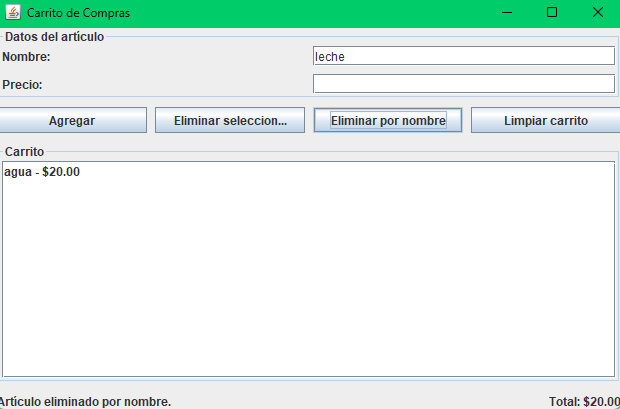
\includegraphics[width=\linewidth]{Imagenes/nombre.png}
        \caption*{Eliminar artículos por nombre}
    \end{subfigure}
    \hfill
    \begin{subfigure}{0.45\textwidth}
        \centering
        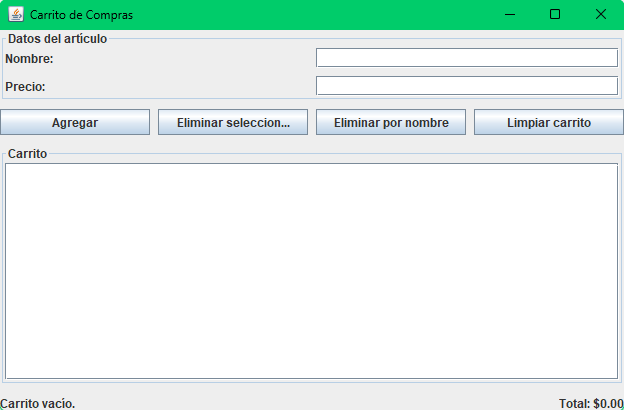
\includegraphics[width=\linewidth]{Imagenes/vaciar.png}
        \caption*{Vaciar carrito}
    \end{subfigure}
\end{figure}

\clearpage

\section{Conclusiones}

A través de esta práctica, logramos consolidar nuestros conocimientos sobre el manejo de objetos en Java. Pusimos especial atención a la encapsulación, asegurándonos de que los atributos de las clases estuvieran protegidos y solo se accediera a ellos mediante métodos designados. Además, también comprendimos sobre la relevancia del empaquetamiento como estrategia clave para una buena organización del código y su posterior mantenimiento. La simulación del carrito de compras sirvió como un excelente ejemplo de pruebas, pues nos permitió implementar operaciones básicas como la adición, eliminación y visualización de artículos en un entorno gráfico. Definitivamente, esta experiencia consolidó nuestra visión sobre el diseño modular en Java y la importancia de una interacción segura entre clases para crear aplicaciones más estructuradas y funcionales.

\printbibliography

\clearpage

\section{Reto para token}

Para realizar este reto, reutilizamos las clases \textbf{Vista} y \textbf{MainApp}, cambiando los botones y los frames, que es donde se muestra el texto. En la clase \textbf{MainApp} cambiamos los listeners, poniendo que pasa en cada caso, utilizamos listas que guardaran tanto los números como las operaciones, y al darle igual, se calculara lo que hay dentro de esas listas.

Utilizamos banderas para resolver los errores que nos salían en el programa.

\begin{figure}[H]
    \centering
    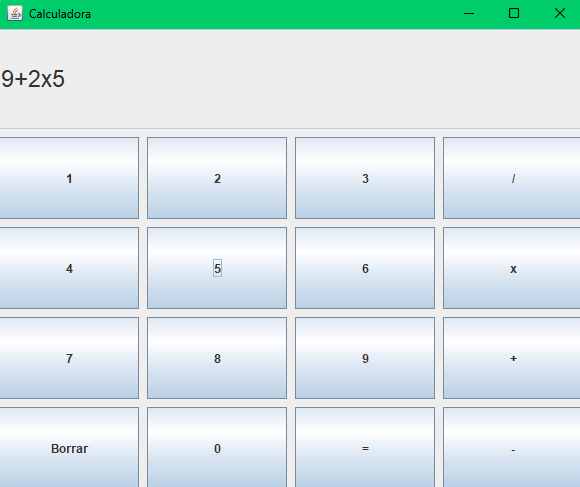
\includegraphics[width=0.4\linewidth]{Imagenes/calculadora1.png}
    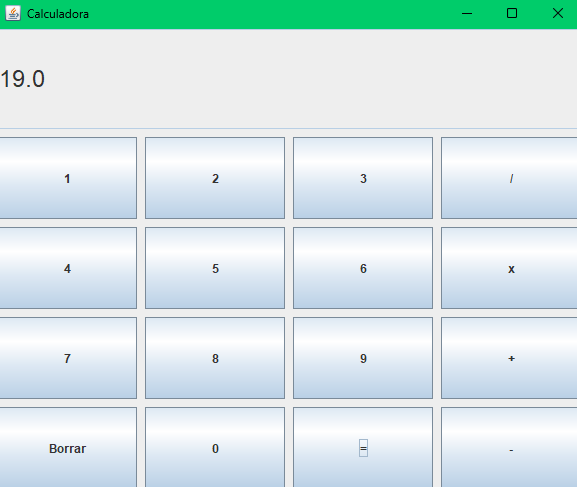
\includegraphics[width=0.4\linewidth]{Imagenes/calculadora2.png}
    \caption*{Ejecución de la calculadora}
\end{figure}

\end{document}